\documentclass[12pt,a4paper]{report}
\usepackage{fontspec}
\usepackage{fullpage}
\usepackage{hyperref}
\usepackage{array}
\usepackage{url}
\usepackage{amsmath}
\usepackage{pgfplotstable}
\usepackage{algorithm2e}
\usepackage{multirow}
\usepackage{subcaption}
\usepackage{color}
\usepackage{adjustbox}
\usepackage{tikz}
\usepackage{tikz-dependency}
\usepackage{titling}
\usepackage{pdfpages}
\usepackage{setspace}
\usepackage[round]{natbib}
\usetikzlibrary{shapes,fit,calc,er,positioning,intersections,decorations.shapes,mindmap,trees}
\tikzset{decorate sep/.style 2 args={decorate,decoration={shape backgrounds,shape=circle,
      shape size=#1,shape sep=#2}}}

\newfontfamily\hebfont[Script=Hebrew, Scale=MatchUppercase]{FreeSans}
\newcommand{\heb}[1]{\bgroup\textdir TRT\hebfont #1\egroup}

\title{
\textbf{Universal Semantic Parsing with Neural Networks} \\
\vspace{2cm}
{\large Thesis submitted for the degree of \\
``Doctor of Philosophy''}
}
\author{
By \\
Daniel Hershcovich
\vspace{2cm}
}
\date{
Submitted to the Senate of the Hebrew University \\
February, 2019
}

\onehalfspacing

\begin{document}

\maketitle
\maketitle
\clearpage
\title{}
\author{
This work was carried out under the supervision of: \\
Prof. Ari Rappoport and Dr. Omri Abend
}
\date{}
\maketitle

\section*{Acknowledgments}

Even before I started my studies at the PhD program of
the Edmond and Lily Safra Center for Brain Sciences
(then the Interdisciplinary Center for Neural Computation),
I was interested in human language in general and learning languages
in particular, an interest I found early on that I shared with who became
my (first) PhD advisor, Ari Rappoport, to whom I am grateful for the
insightful conversations all along this process.
I am of course also indebted to my second advisor, Omri Abend,
whose shared interests with me and Ari have led to a fruitful
research project, which is still ongoing and I hope will continue for
many years.
They have set a very high standard, to which I continuously strive
and to which I surely owe much of my success so far.
I also thank my PhD committee members, Roi Reichart and Yoav Goldberg,
whose invaluable advice has shaped my research direction in the best way possible.

I sincerely appreciate the support of the ELSC staff and students,
and particularly the members of my year,
Adar Adamsky, Yonatan Bain, Haran Shani, Matan Holtzer, Henrike Horn, Adi Kol,
Ori Lavi Rotbain, Nimrod Levin, Oren Peles, Pnina Rappel, Benjamin Weiner, and
Noga Zaslavsky, whose company since the early stages of my graduate studies
has given me a sense of belonging and comfort.
I also thank the many other friends I made during my studies, including Nora Vrieler,
Ana Polterovich, Johannes Niediek, Dan Valsky, Nova Fandina and Stav Yardeni,
for their support.

My gratitude also goes to Roy Schwartz, who shared a great deal of his
experience with me and helped me become confident in my ideas, and to
Elior Sulem, who has accompanied me as a student in the lab and with whom
I shared a considerable part of my time there.
I would also like to thank past and current lab members, including Oren Tsur,
Eva Kimel, Dana Rubinstein, Saggy Herman, Effi Levi, Leshem Choshen, Zohar Aizenbud,
Aviram Stern, Adi Bitan and Michal Kessler, who have made these few years both
pleasant and interesting.
I must also express my gratitude towards Dotan Dvir and the UCCA annotation team,
without which this work would simply not have been possible.

Finally, I owe my deepest gratitude to my family for their support along the way,
and to my partner Michal for her endless love, patience and understanding,
which I value greatly.

\pagebreak

\section*{Abstract}

Natural language processing (NLP) is a scientific and technological field
concerned with developing methods for performing linguistic tasks automatically.
These include classifying text into categories,
tagging it for linguistic properties (such as part-of-speech),
building graphical representations for it
and generating new text according to some constraints.
For example, \textit{machine translation} is the task of generating
text in a target language given source language text.

A major effort in NLP is dedicated to \textit{natural language understanding},
which aims to be able to comprehend text, reason about it, and act upon it
in an intelligent way.
While specific use-cases or benchmarks can be solved with relatively simple
systems, which either ignore word order (``bag-of-words'' models) or treat
it as a simple linear structure
(such as the popular sequence-to-sequence framework allowing neural networks
to learn tasks in an end-to-end fashion),
understanding human language in general
requires a hierarchical representation of meaning.
Constructing this representation from text has been the goal of an extensive
line of work in \textit{semantic parsing}.
While many semantic representation schemes have been proposed,
they share many of their basic distinctions, such as between predicates
(relations, states and events) and arguments (participants).

This thesis focuses on a particular semantic representation scheme called
\textit{Universal Conceptual Cognitive Annotation} (UCCA),
whose main design principles are support for all major linguistic semantic phenomena,
cross-linguistic applicability and stability across translations,
ease of annotation (even by those who are not experts in linguistics),
and a modular architecture supporting multiple layers of semantic annotation.
A fully automatic parser is presented, and evaluated on multiple languages
(English, French and German).
The parser, titled ``TUPA'' (transition-based UCCA parser),
is able to learn very general graph structures:
directed acyclic graphs over token sequences with non-terminal nodes for complex
units, where these may cover discontinuous terminal yields.
This general class of graphs covers the structures annotated in UCCA,
as well as other representation schemes.
TUPA is implemented as a transition-based parser, whose transition system
supports these structural properties.
Its transition classifier is a neural network equipped with a
bidirectional long short-term memory (BiLSTM) module for calculating
feature representations for the input.
In an extensive comparison to conversion-based methods, as well as
other classifier implementations, TUPA is shown to outperform all baselines
in the task of UCCA parsing in both in-domain and out-of-domain settings
in three languages.

The parser is subsequently applied to two other semantic representation schemes,
DM and AMR, and to syntactic dependencies in the Universal Dependencies (UD)
scheme. This demonstrates that the flexible parser is usable not just for UCCA
parsing.
Furthermore, training TUPA in a multitask setting on all of these schemes
improves its UCCA parsing accuracy, by effectively learning generalizations
across the different representations.

Finally, in an empirical comparison of
the content of semantic and syntactic representations, we discover several
aspects of divergence.  These have profound impact on the potential
contribution of syntax to semantic parsing, and on the usefulness of each of
the approaches for semantic tasks in natural language processing.

\pagebreak

\tableofcontents

\chapter{Introduction}

Natural language processing (NLP) or computational linguistics (CL)
is a sub-field of computer science with two main goals:
(1) developing methods for performing linguistic tasks automatically
so that solutions can be engineered for better human-computer interface
or analysis of large amounts of natural language data;
(2) computational modeling and study of natural language to answer linguistic questions.

Applications in NLP include classifying text into categories
(such as spam/non-spam, by topic, by author properties, or by
the sentiment expressed in it),
tagging it for linguistic properties (such as part-of-speech, i.e., noun/verb/etc.),
building abstract representations for it (for linguistic research or for
more readily integrating them into downstream applications)
and generating new text according to some constraints (for example,
machine translation is the task of generating
text in a target language given source language text;
text simplification is the task of generating simple text with approximately the same
meaning as given complex text).

Semantic tasks in natural language processing, such as machine translation and
sentiment analysis, require understanding the meaning of text. Since text is
merely a sequence of words, it has to be represented in a way that will convey
its meaning. One simple approach, known as the bag-of-words model, looks only
at which words occur in the text.
This can already provide
substantial information about the meaning, but it ignores the order of words,
which clearly conveys important information as well. The n-gram model counts
sequences of words with regard to their order, incorporating at least some of
the meaning encoded in the text structure.
Many models treat text as a simple linear structure,
such as the popular sequence-to-sequence framework allowing neural networks
to learn tasks in an end-to-end fashion.

Specific use-cases or benchmarks can be solved with such relatively simple
systems, which either ignore word order or make simplifying assumptions about structure.
However, understanding human language in general
requires a hierarchical representation of meaning,
as an undeniable part in the
meaning of language resides in its hierarchical structure.

Indeed, a major effort in NLP is dedicated to \textit{natural language understanding},
which aims to be able to comprehend text, reason about it, and act upon it
in an intelligent way.
For example, executable semantic parsing\footnote{Two conceptually distinct
tasks are termed \textit{semantic parsing}: parsing into
executable representations, such as SQL; and parsing into descriptive meaning
representation, such as AMR or UCCA.
We disambiguate by referring to the former as \textit{executable semantic parsing}.}
is the task of generating logical meaning representations in the form of code, such as
SQL or Python, which can then be executed against a knowledge base to perform
tasks or answer questions.
In general, constructing a hierarchical representation from text has been the
goal of an extensive line of work in \textit{semantic parsing}.
While many semantic representation schemes have been proposed,
they share many of their basic distinctions \citep{abend2017state},
such as between predicates
(relations, states and events) and arguments (participants).

Syntax is a way to
model this structure formally. Using syntactic features can improve the
performance in semantic tasks.
However, syntactic annotations suffer from limitations, since they do not
represent the semantic structure of text directly. Simple manipulations such as
switching from an active construction to a passive one, which nearly do not
alter the meaning of text, can yield a significantly different syntactic
structure. Moreover, the same syntactic construct can express conceptually
distinct semantic structures: while ``chairmen of parliaments'' and
``dozens of parliaments'' have the same syntactic structure, semantically
they are quite distinct.

Universal Dependencies \citep{nivre2016universal}
is a \textit{syntactic} dependency scheme aiming for cross-lingual consistency,
whose annotation is often similar to the common practice in semantic treebanks
(Figure~\ref{fig:original_example_ud}).

\begin{figure}[t]
  \centering
    \begin{dependency}[text only label, label style={above,font=\tt}, font=\small]
    \begin{deptext}[column sep=.8em,ampersand replacement=\^]
    After \^ graduation \^ , \^ John \^ moved \^ to \^ Paris \\
    \end{deptext}
        \depedge[edge unit distance=1ex]{2}{1}{case}
        \depedge[edge unit distance=1ex]{2}{3}{punct}
        \depedge[edge unit distance=1ex]{5}{4}{nsubj}
        \depedge[edge unit distance=1ex, edge end x offset=-2pt]{5}{2}{obl}
        \depedge[edge unit distance=1ex]{7}{6}{case}
        \deproot[edge unit distance=1.5ex]{5}{root}
        \depedge[edge unit distance=1.5ex]{5}{7}{obl}
    \end{dependency}
\caption{Example UD tree, demonstrating practices common in semantic annotation:
linking content words to content words, and preference of lexical heads over functional ones.
\label{fig:original_example_ud}}
\end{figure}

Semantic annotation schemes attempt to represent the meaning of natural
language utterances directly. An example is semantic role
labeling, which annotates
predicates and their arguments, classifying them into specific roles. As
opposed to syntactic annotation, which reflects language-specific formal
patterns, semantic annotation corresponds to a higher level of cognitive
processing, and the same framework can potentially apply to any language.
Moreover, a rich semantic annotation scheme may be better than
syntactic annotation as an input for applications that attempt to solve a
semantic task, due to their tighter relation to the meaning of the text.

While earlier work on semantic parsing has mostly concentrated on shallow semantic analysis,
focusing on semantic role labeling of verbal argument structures,
the focus has recently shifted to parsing of more elaborate representations that account
for a wider range of phenomena. 
Most closely related to my work is Broad-Coverage Semantic Dependency Parsing (SDP).
It addresses a wide range of semantic phenomena,
and supports discontinuous units and multiple parents \cite{oepen2016towards}.
However, SDP uses bi-lexical dependencies
(meaning every relation or edge is between a pair of words),
disallowing non-terminal nodes (see below),
and thus faces difficulties in supporting
structures that have no clear head, such as coordination \cite{Ivanova2012who}.

Another line of work addresses parsing into Abstract Meaning Representations (AMRs)
\cite{banarescu2013abstract,flanigan2014discriminative,vanderwende2015amr,pust2015parsing,artzi2015broad}. 
While sharing much of my work's motivation,
AMR does not ground its units in the words and constituents of the text.
This complicates the parsing task, as it requires
that the alignment between words and logical symbols be automatically
(and imprecisely) detected.
\cite{wang2015transition} applied a transition-based approach to AMR parsing,
but their method involved first syntactically parsing the input, and then converting
the resulting tree into an AMR.

Semantic parsing methods can be largely partitioned into grammar-based and grammarless methods.
Within the grammar-based literature, most work relied on Combinatory Categorial Grammar (CCG)
\cite{Steedman:00}, which allows computing semantic structure compositionally from the
syntactic derivations. Notable examples include the Boxer parser \cite{bos2005towards}
and the AMR parser by \cite{artzi2015broad}.
Other examples include parsing with Hyperedge Replacement Grammars
\cite{jones2012semantics}.
A different line of work takes a discriminative, grammarless approach,
pursuing either graph-based methods that predict the highest ranking graph
(tree or DAG) that satisfies a given set of constraints
\cite[for AMR parsing]{flanigan2014discriminative},
or a transition-based method
that builds the parse incrementally following a series of local
decisions \cite{Nivre03anefficient}.

In order to represent the full range of semantic structures exhibited by
natural language, three properties should be supported: reentrancy,
representing arguments shared between predicates;
non-terminal nodes for multi-word units;
and discontinuity of semantic units in the text.

The first property, \textbf{reentrancy} (or \textbf{multiple parents}), is required for
representing arguments and relations (semantic units) that are shared between predicates.
For instance, in the sentence
``After graduation, John moved to Paris'' (Figure~\ref{fig:graduation}),
``John'' is an argument of both ``graduation''
and ``moved'', yielding a DAG structure rather than a tree.

The second is \textbf{non-terminal nodes} for representing units
comprising more than one word (Figure~\ref{fig:home}).
While bi-lexical dependencies partially circumvent this requirement, by
representing complex units in terms of their headwords, they fall short
when representing units that have no clear head.
Frequent examples of such constructions include
coordination structures (e.g., ``\textit{John and Mary} went home''),
some multi-word expressions (e.g., ``The Haves and the \textit{Have Nots}''),
and prepositional phrases.
In these cases, dependency schemes often apply some annotation convention that
selects one of the sub-units
as the head, but as different head selections are needed for different purposes,
standardization problems arise \cite{Ivanova2012who}.
For example, selecting the preposition to head prepositional phrases yields better
parsing results \cite{Schwartz:12}, while the head noun can be more useful for
information extraction purposes.

Third, semantic units may be \textbf{discontinuous} in the text. For instance, in
``John \textit{gave} everything \textit{up}'' (Figure~\ref{fig:gave}),
the phrasal verb ``gave ... up'' forms a single semantic unit.
Discontinuities are also pervasive with other multi-word
expressions \cite{schneider2014discriminative}.

\begin{figure}[h]\small\centering
  \begin{subfigure}{\textwidth}\centering
  \parbox{.1\textwidth}{\caption{}\label{fig:graduation}}
  \parbox{.4\textwidth}{
  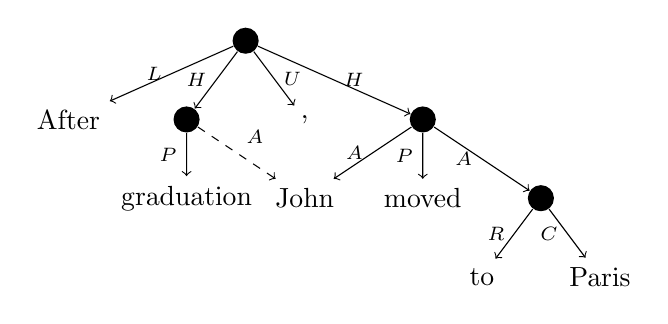
\begin{tikzpicture}[level distance=10mm, ->]
    \node (ROOT) [fill=black, circle] {}
      child {node (After) {After} edge from parent node[left] {\scriptsize $L$}}
      child {node (graduation) [fill=black, circle] {}
      {
        child {node {graduation} edge from parent node[left] {\scriptsize $P$}}
      } edge from parent node[left] {\scriptsize $H$} }
      child {node {,} edge from parent node[right] {\scriptsize $U$}}
      child {node (moved) [fill=black, circle] {}
      {
        child {node (John) {John} edge from parent node[left] {\scriptsize $A$}}
        child {node {moved} edge from parent node[left] {\scriptsize $P$}}
        child {node [fill=black, circle] {}
        {
          child {node {to} edge from parent node[left] {\scriptsize $R$}}
          child {node {Paris} edge from parent node[left] {\scriptsize $C$}}
        } edge from parent node[left] {\scriptsize $A$} }
      } edge from parent node[right] {\scriptsize $H$} }
      ;
    \draw[dashed,->] (graduation) to node [auto] {\scriptsize $A$} (John);
  \end{tikzpicture}
  }
  \end{subfigure}
  \begin{subfigure}{\textwidth}\centering
  \parbox{.1\textwidth}{\caption{}\label{fig:home}}
  \parbox{.4\textwidth}{
  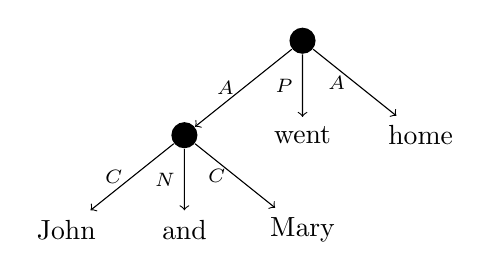
\begin{tikzpicture}[level distance=12mm, ->,
      every node/.append style={midway}]
    \node (ROOT) [fill=black, circle] {}
      child {node [fill=black, circle] {}
      {
        child {node {John} edge from parent node[left] {\scriptsize $C$}}
        child {node {and} edge from parent node[left] {\scriptsize $N$}}
        child {node {Mary} edge from parent node[left] {\scriptsize $C$}}
      } edge from parent node[left] {\scriptsize $A$} }
      child {node {went} edge from parent node[left] {\scriptsize $P$}}
      child {node {home} edge from parent node[left] {\scriptsize $A$}}
      ;
  \end{tikzpicture}
  }
  \end{subfigure}
  \begin{subfigure}{\textwidth}\centering
  \parbox{.1\textwidth}{\caption{}\label{fig:gave}}
  \parbox{.4\textwidth}{
  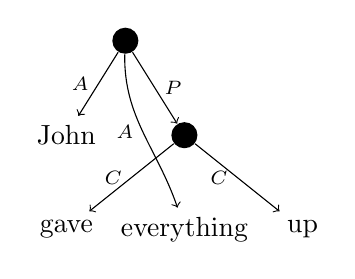
\begin{tikzpicture}[level distance=12mm, ->,
      every node/.append style={midway}]
    \node (ROOT) [fill=black, circle] {}
      child {node {John} edge from parent node[left] {\scriptsize $A$}}
      child {node [fill=black, circle] {}
      {
      	child {node {gave} edge from parent node[left] {\scriptsize $C$}}
      	child {node (everything) {everything} edge from parent[white]}
      	child {node {up} edge from parent node[left] {\scriptsize $C$}}
      } edge from parent node[right] {\scriptsize $P$} }
      ;
    \draw[bend right,->] (ROOT) to[out=-20, in=180] node [left] {\scriptsize $A$} (everything);
  \end{tikzpicture}
  }
  \end{subfigure}
  \begin{subfigure}{\textwidth}\centering
  \parbox{.1\textwidth}{\caption{}\label{fig:shower}}
  \parbox{.4\textwidth}{
  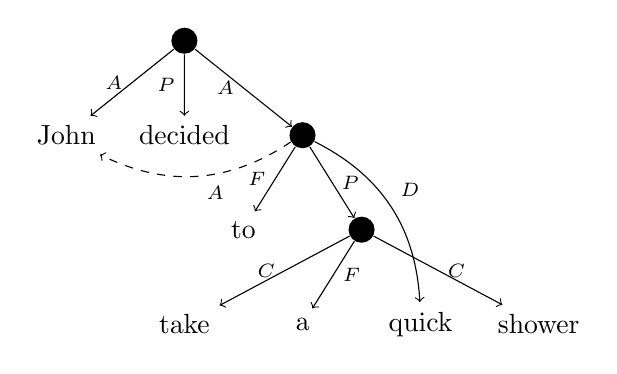
\begin{tikzpicture}[level distance=12mm, ->,
      every node/.append style={midway}]
    \node (ROOT) [fill=black, circle] {}
      child {node (John) {John} edge from parent node[left] {\scriptsize $A$}}
      child {node {decided} edge from parent node[left] {\scriptsize $P$}}
      child {node (totakeaquickshower) [fill=black, circle] {}
      {
        child {node {to} edge from parent node[left] {\scriptsize $F$}}
        child {node [fill=black, circle] {}
        {
          child {node {take} edge from parent node[left] {\scriptsize $C$}}
          child {node {a} edge from parent node[right] {\scriptsize $F$}}
          child {node (quick) {quick} edge from parent[white]}
          child {node {shower} edge from parent node[right] {\scriptsize $C$}}
        } edge from parent node[right] {\scriptsize $P$} }
      } edge from parent node[left] {\scriptsize $A$} }
      ;
    \draw[bend left,dashed,->] (totakeaquickshower) to node [auto] {\scriptsize $A$} (John);
    \draw[bend left,->] (totakeaquickshower) to node [auto] {\scriptsize $D$} (quick);
  \end{tikzpicture}
  }
  \end{subfigure}
  \caption{\label{fig:examples}
    UCCA examples.
    (\subref{fig:graduation}) includes a remote edge (dashed),
    resulting in ``John'' having two parents.
    (\subref{fig:home}) includes a coordination construction (``John and Mary'').
    (\subref{fig:gave}) includes a discontinuous unit (``gave ... up'').
    (\subref{fig:shower}) includes both a remote edge and a discontinuous unit (``take a ... shower'').
    Legend: $P$ -- Process (a Scene's main relation), $A$ -- Participant,
    $L$ -- inter-scene Linker, $H$ -- Parallel Scene, $C$ -- Center, $D$ -- Adverbial,
    $R$ -- Relator, $N$ -- Connector, $U$ -- Punctuation, $F$ -- Function unit.
  }
\end{figure}

The only semantic annotation scheme that supports the combination of these criteria is UCCA
\citep{abend2013universal}:
Universal Cognitive Conceptual Annotation
is a cross-linguistically applicable semantic representation scheme.
It covers the predicate-argument
structures evoked by predicates of all grammatical categories, the inter-relations between them,
as well as other major linguistic phenomena.
UCCA has demonstrated applicability to multiple languages,
rapid annotation \citep{abend2017uccaapp},
stability in translation \citep{sulem2015conceptual}
and benefit for various applications:
evaluation of machine translation \citep{birch2016hume},
evaluation of grammatical error correction \citep{choshen2018reference},
evaluation of structural text simplification \citep{sulem2018semantic},
and text simplification \citep{sulem2018simple}.

My research is concerned with learning to parse UCCA graphs from text, representing its semantics.
I introduce a general graph parser,
and investigate the relationship with other representations to find beneficial commonalities and
differences highlighting the potential utility of semantic parsers for text understanding applications.
The analysis also exposes challenges semantic parsers must address,
and potential sources for improvement.

To summarize, this thesis has the following goals:
developing techniques for general graph parsing, and
specifically, devising a method for automatic prediction of UCCA
    structure given plain text;
investigating and quantifying the relationship between the content
    captured in UCCA and other semantic or syntactic representations;
and taking advantage of the similarities to other schemes,
    to improve UCCA parsing by learning common distinctions.

\chapter{Methodology}

\subsection*{Transition-Based Parsing}

Transition-based parsers \citep{Nivre03anefficient} build trees or graphs
as they scan the text incrementally.
The parse is created by applying a \textit{transition} at each step to the parser state,
defined using a buffer of tokens and nodes to be processed,
a stack of nodes currently being processed,
and a graph of constructed nodes and labeled edges.
A classifier is used at each step to select the next transition based on features
that encode the parser's current state.
During training, an oracle creates training instances for the classifier,
based on the gold-standard annotation.

The transition-based approach has produced some of the best
results in syntactic dependency parsing
\citep{kiperwasser2016simple,andor2016globally}, and has also demonstrated
strong performance in a variety of other semantic and syntactic settings
\citep{maier2015discontinuous,damonte-17}.
Transition-based methods are a natural starting point for UCCA parsing,
as the set of distinctions it represents is similar in spirit to the distinctions
conveyed by dependency schemes.


\subsection*{Neural Networks}

Neural networks are powerful machine learning models.
They have yielded state-of-the-art results in many fields,
including natural language processing \citep{goldberg2016primer}.
Inspired by the brain's computation mechanism,
artificial neural networks operate on dense input representations
by a combination of linear and non-linear transformations.

Language data is commonly manifested as sequences
(e.g., sentences are sequences of words).
Recurrent neural networks \citep{elman1990finding} allow representing
arbitrarily sized sequences in a fixed-size vector,
without ignoring the structured properties of the input.
A specific flavor called Long Short Term Memory
(LSTM) is very common as it learns relatively long-term dependencies.
A bidirectional recurrent neural network, such as a BiLSTM,
takes into account both the past and future.


\subsection*{Multitask Learning}

Multitask learning \citep{caruana1998multitask} allows exploiting the overlap between tasks
to effectively extend the training data, 
and has greatly advanced with neural networks and representation learning.
It has been used over the years for NLP tasks with varying degrees of similarity.

Neural multitask learning has mostly been effective in tackling formally similar
tasks \citep{P16-2038},
including
multilingual syntactic dependency parsing \citep{Q16-1031,guo2016exploiting},
as well as multilingual \citep{duong2017multilingual},
and cross-domain semantic parsing \citep{herzig-berant:2017:Short,W17-2607}.

Sharing parameters with a low-level task
has shown great benefit for transition-based syntactic parsing
\citep{bohnet2012transition,Zhang2016StackpropagationIR,constant-nivre:2016:P16-1,more2016joint}.
Recent work has achieved state-of-the-art results in multiple NLP tasks
by jointly learning the tasks forming the NLP standard pipeline using 
a single neural model \citep{collobert2011natural,D17-1206},
thereby avoiding cascading errors, common in pipelines.


\subsection*{Evaluation}
Comparing UCCA structures
$G_p=(V_p,E_p,\ell_p)$ and $G_g=(V_g,E_g,\ell_g)$,
over the same sequence of terminals $W = \{w_1,\ldots,w_n\}$
is done as follows.
For an edge $e=(u,v)$ in either graph, its yield $y(e) \subseteq W$ is the
set of terminals in $W$ that are descendants of $v$.
Define the set of \textit{mutual edges} between $G_p$ and $G_g$:
\[
    M(G_p,G_g) =
    \left\{(e_1,e_2) \in E_p \times E_g \;|\;
    y(e_1) = y(e_2) \wedge \ell_p(e_1)=\ell_g(e_2)\right\}
\]

Labeled precision and recall are defined by dividing $|M(G_p,G_g)|$ by $|E_p|$ and $|E_g|$, respectively,
and F-score by taking their harmonic mean.
Two variants are reported: one where we consider only primary edges,
and another for remote edges



\chapter{A Transition-Based Directed Acyclic Graph Parser for UCCA \\ (Published in ACL 2017)}

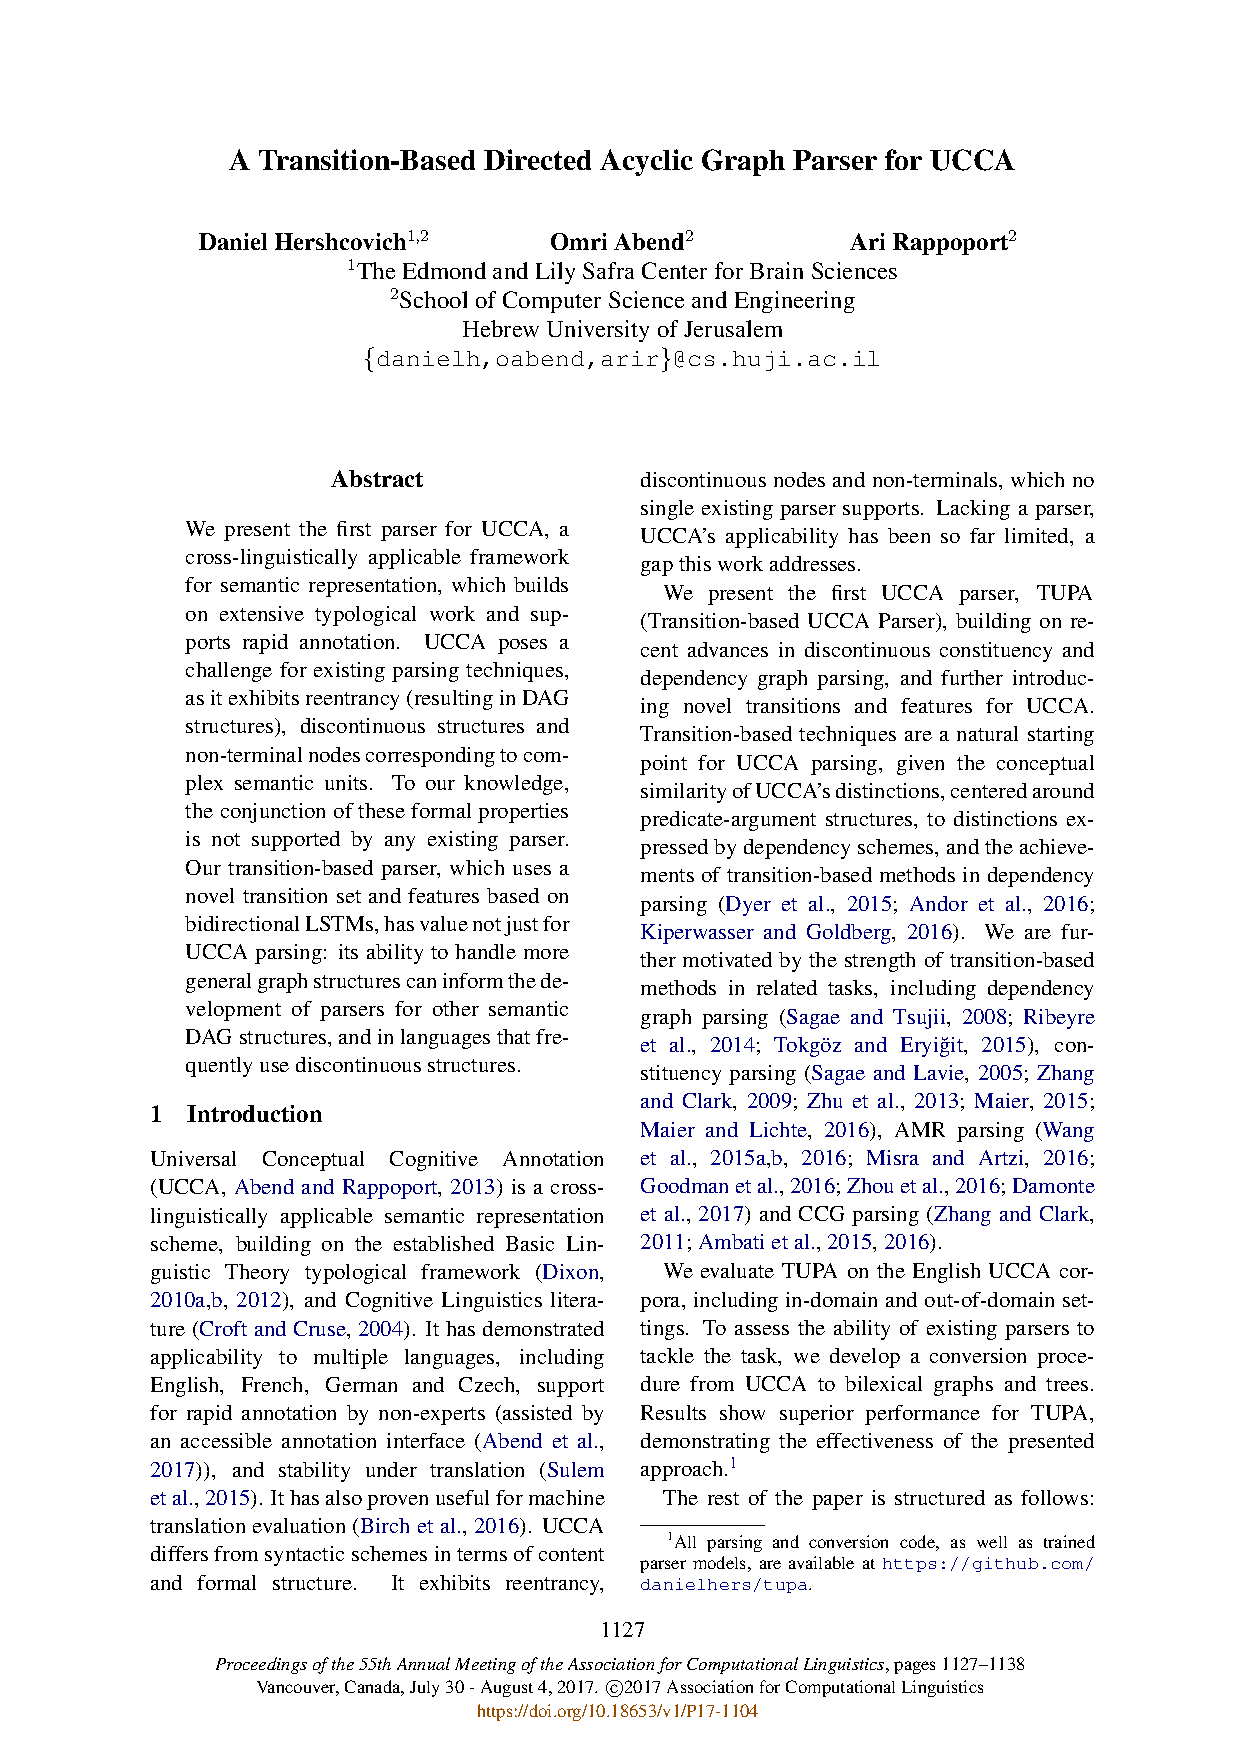
\includepdf[pages=-]{P17-1104.pdf}

\chapter*{A Transition-Based Directed Acyclic Graph Parser for UCCA \\ Supplementary Notes}

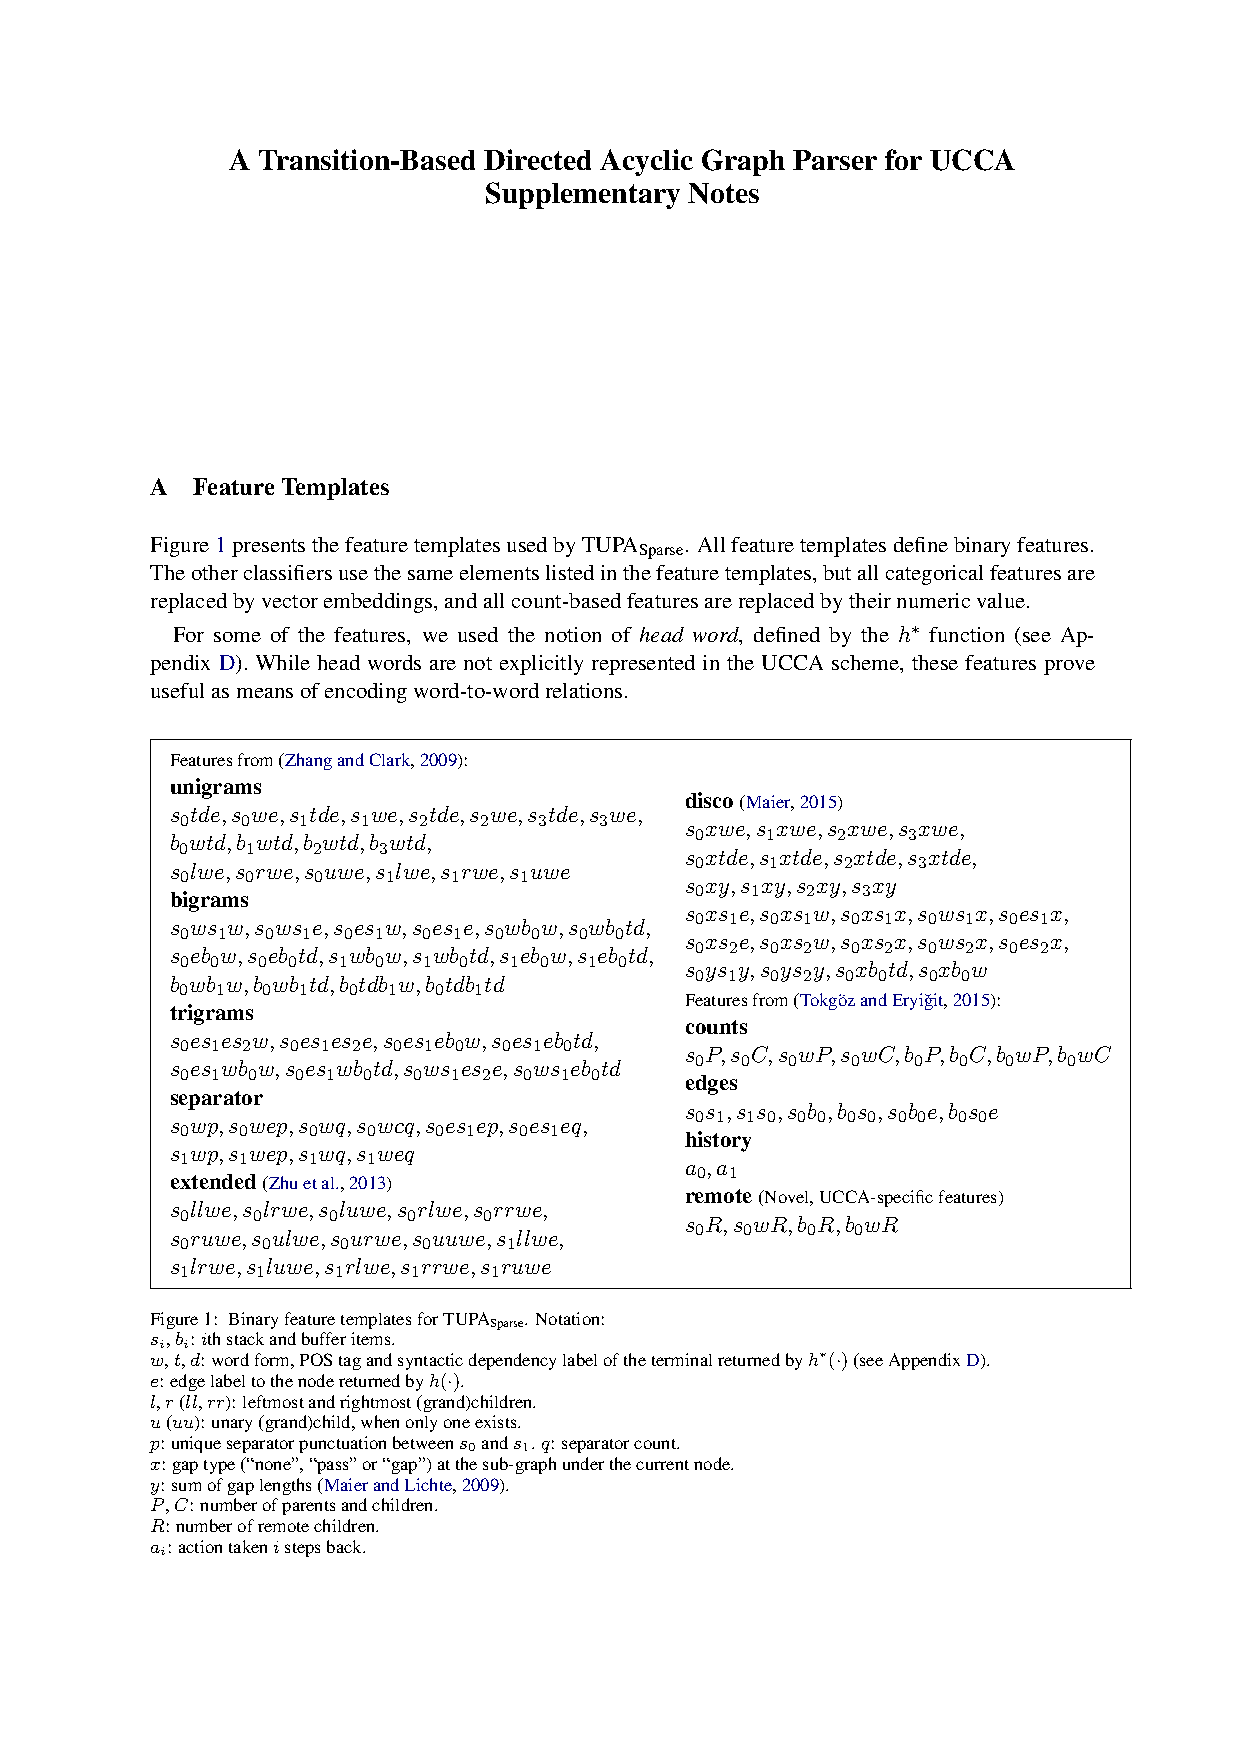
\includepdf[pages=-]{P17-1104_supp.pdf}

\chapter{Multitask Parsing Across Semantic Representations \\ (Published in ACL 2018)}

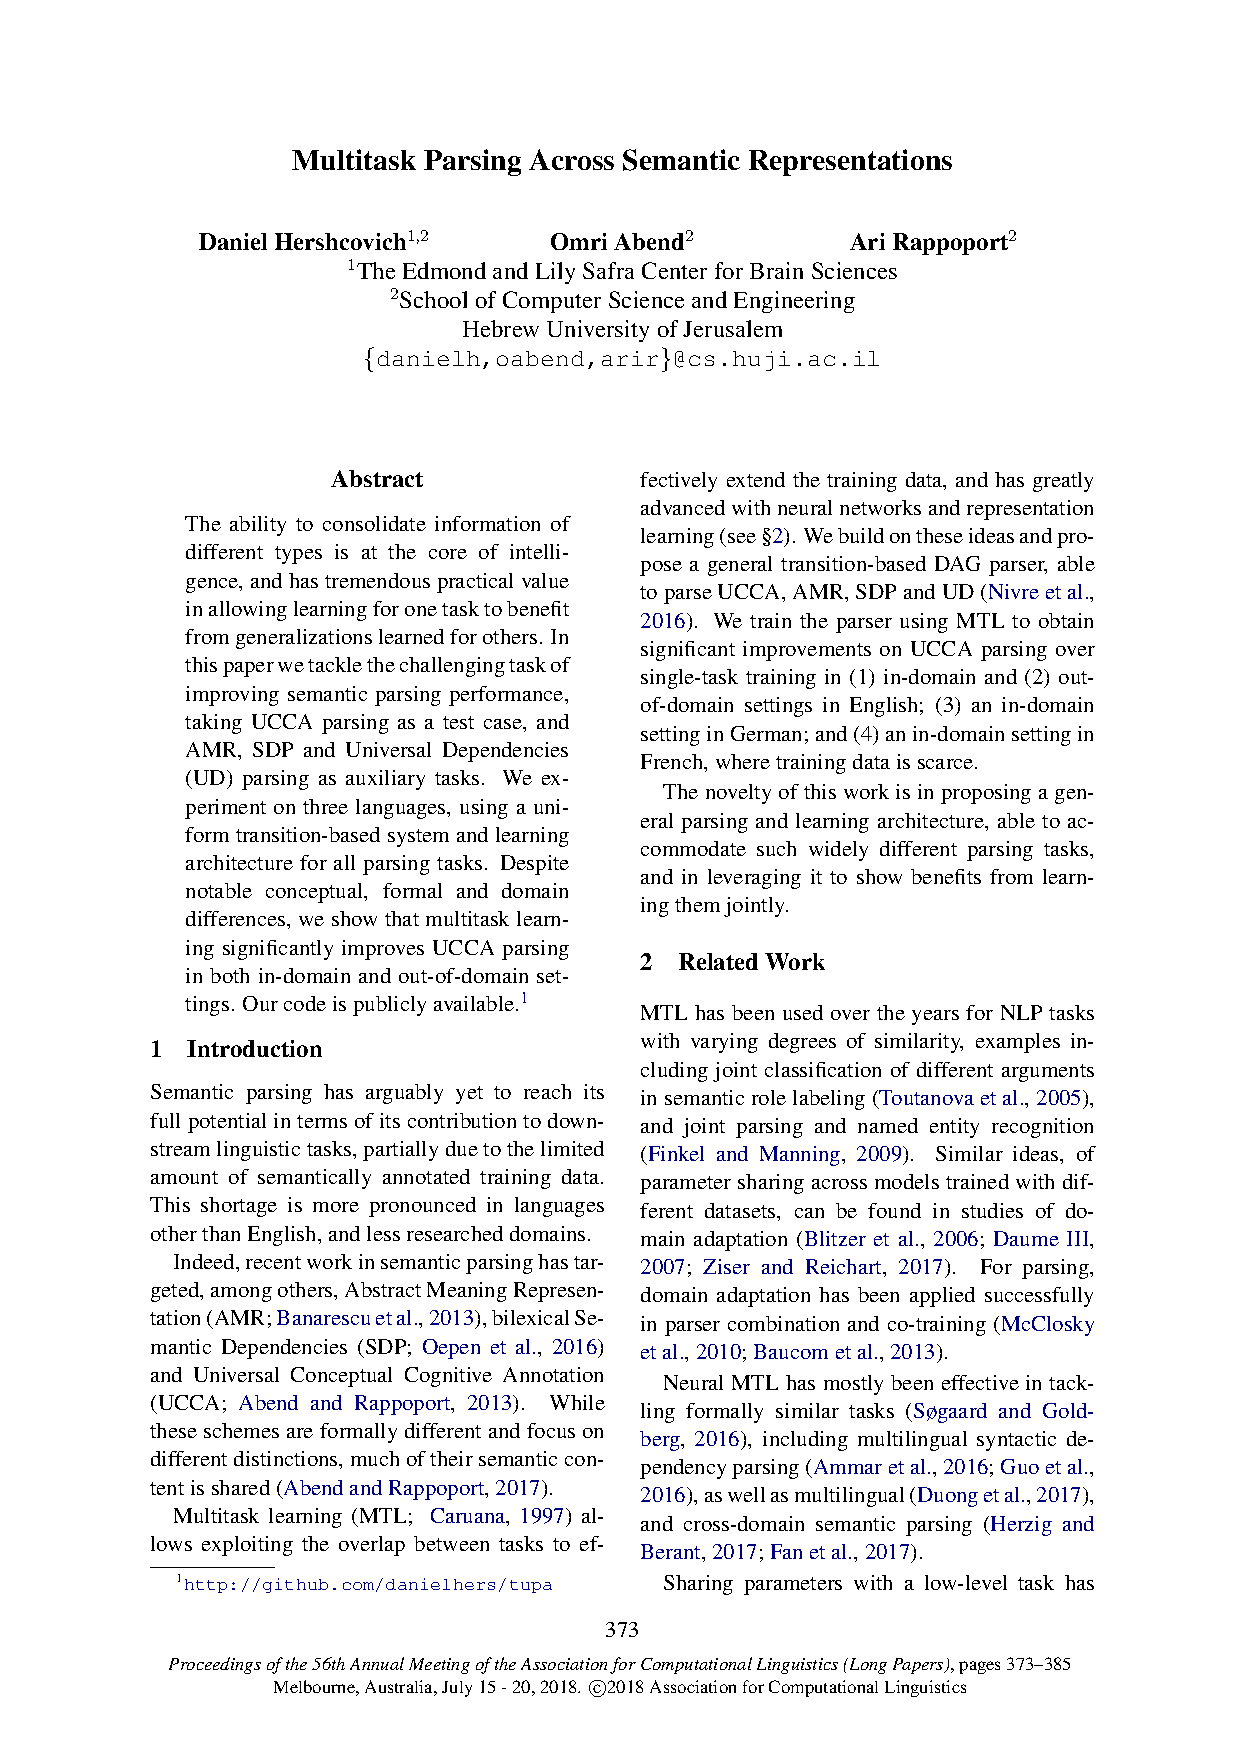
\includepdf[pages=-]{P18-1035.pdf}

\chapter*{Multitask Parsing Across Semantic Representations \\ Supplementary Notes}

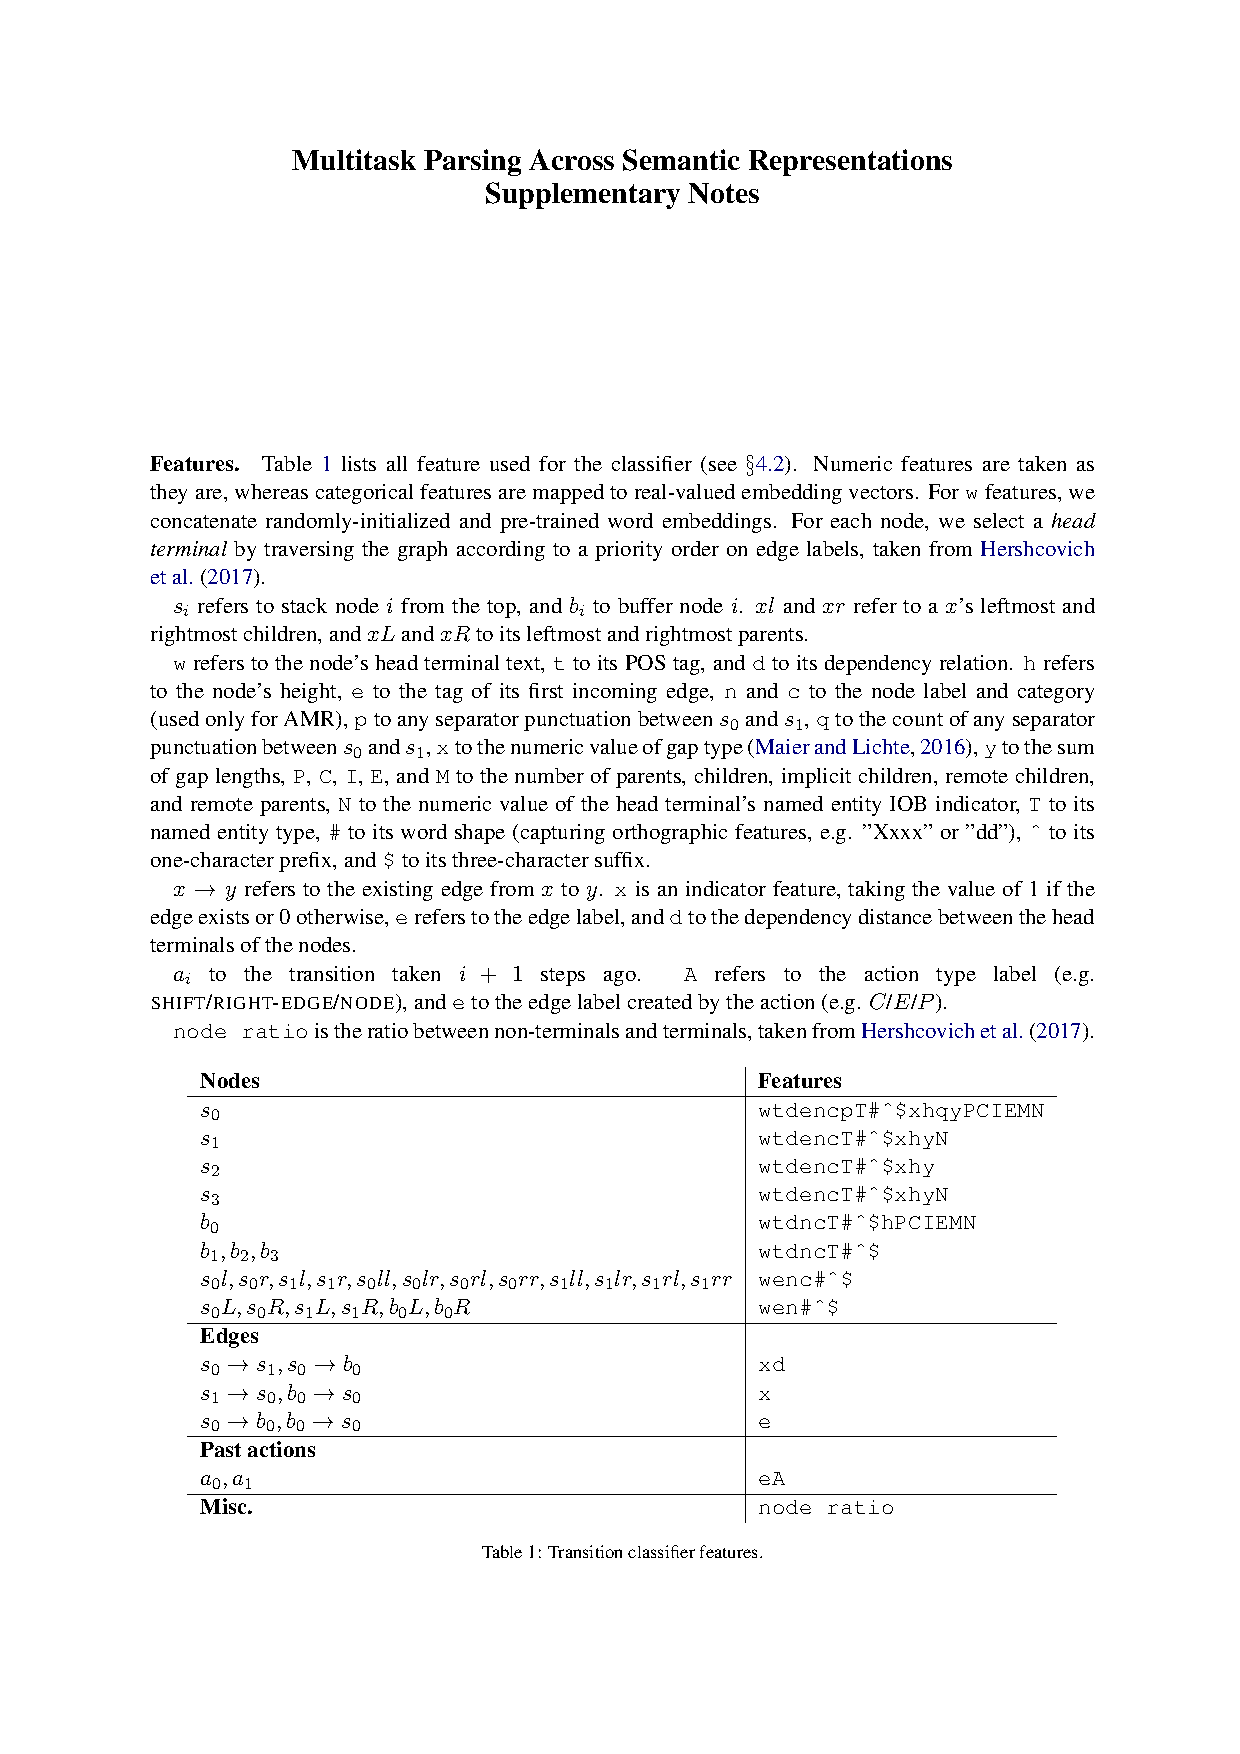
\includepdf[pages=-]{P18-1035_supp.pdf}

\chapter{Universal Dependency Parsing with a General Transition-Based DAG Parser \\ (Published in CoNLL 2018 Shared Task)}

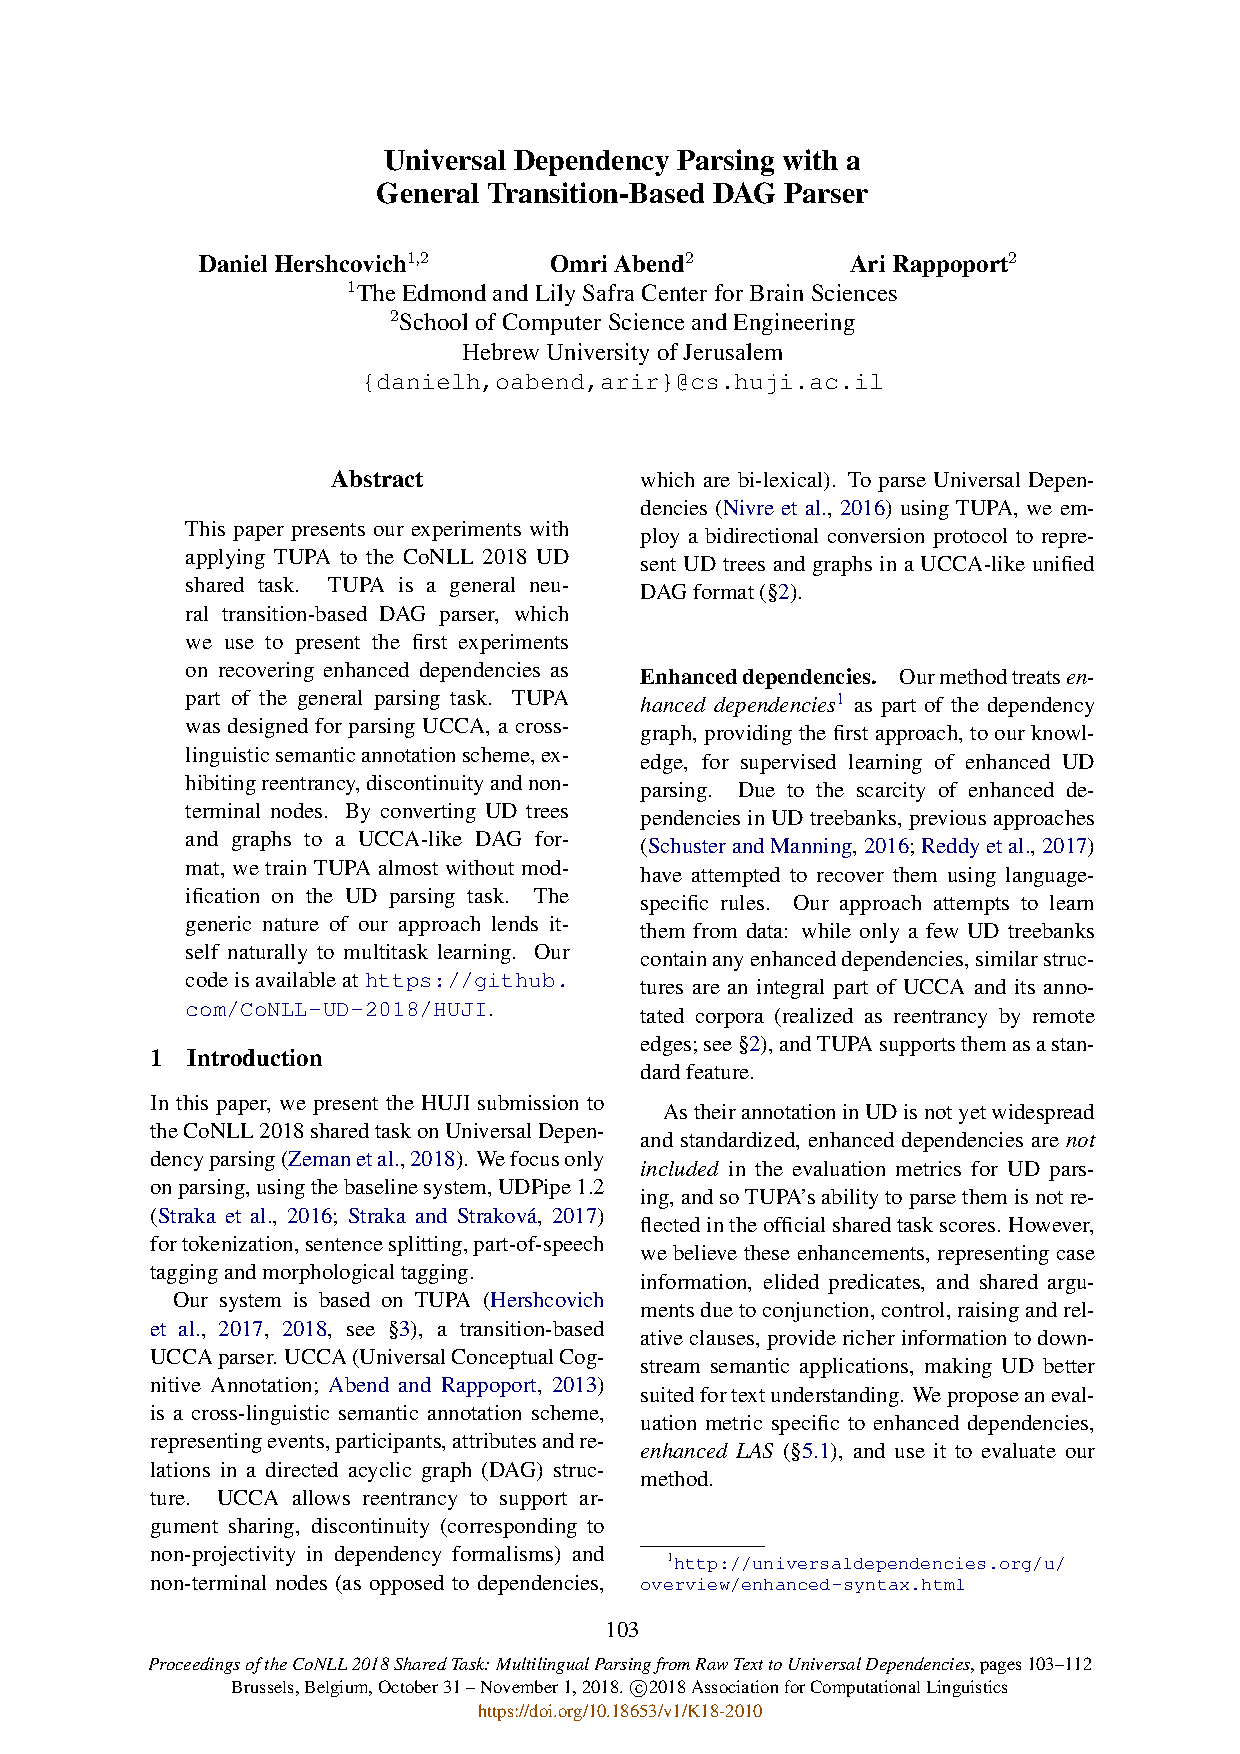
\includepdf[pages=-]{K18-2010.pdf}

\chapter{Content Differences in Syntactic and Semantic Representations \\ (Under Submission)}

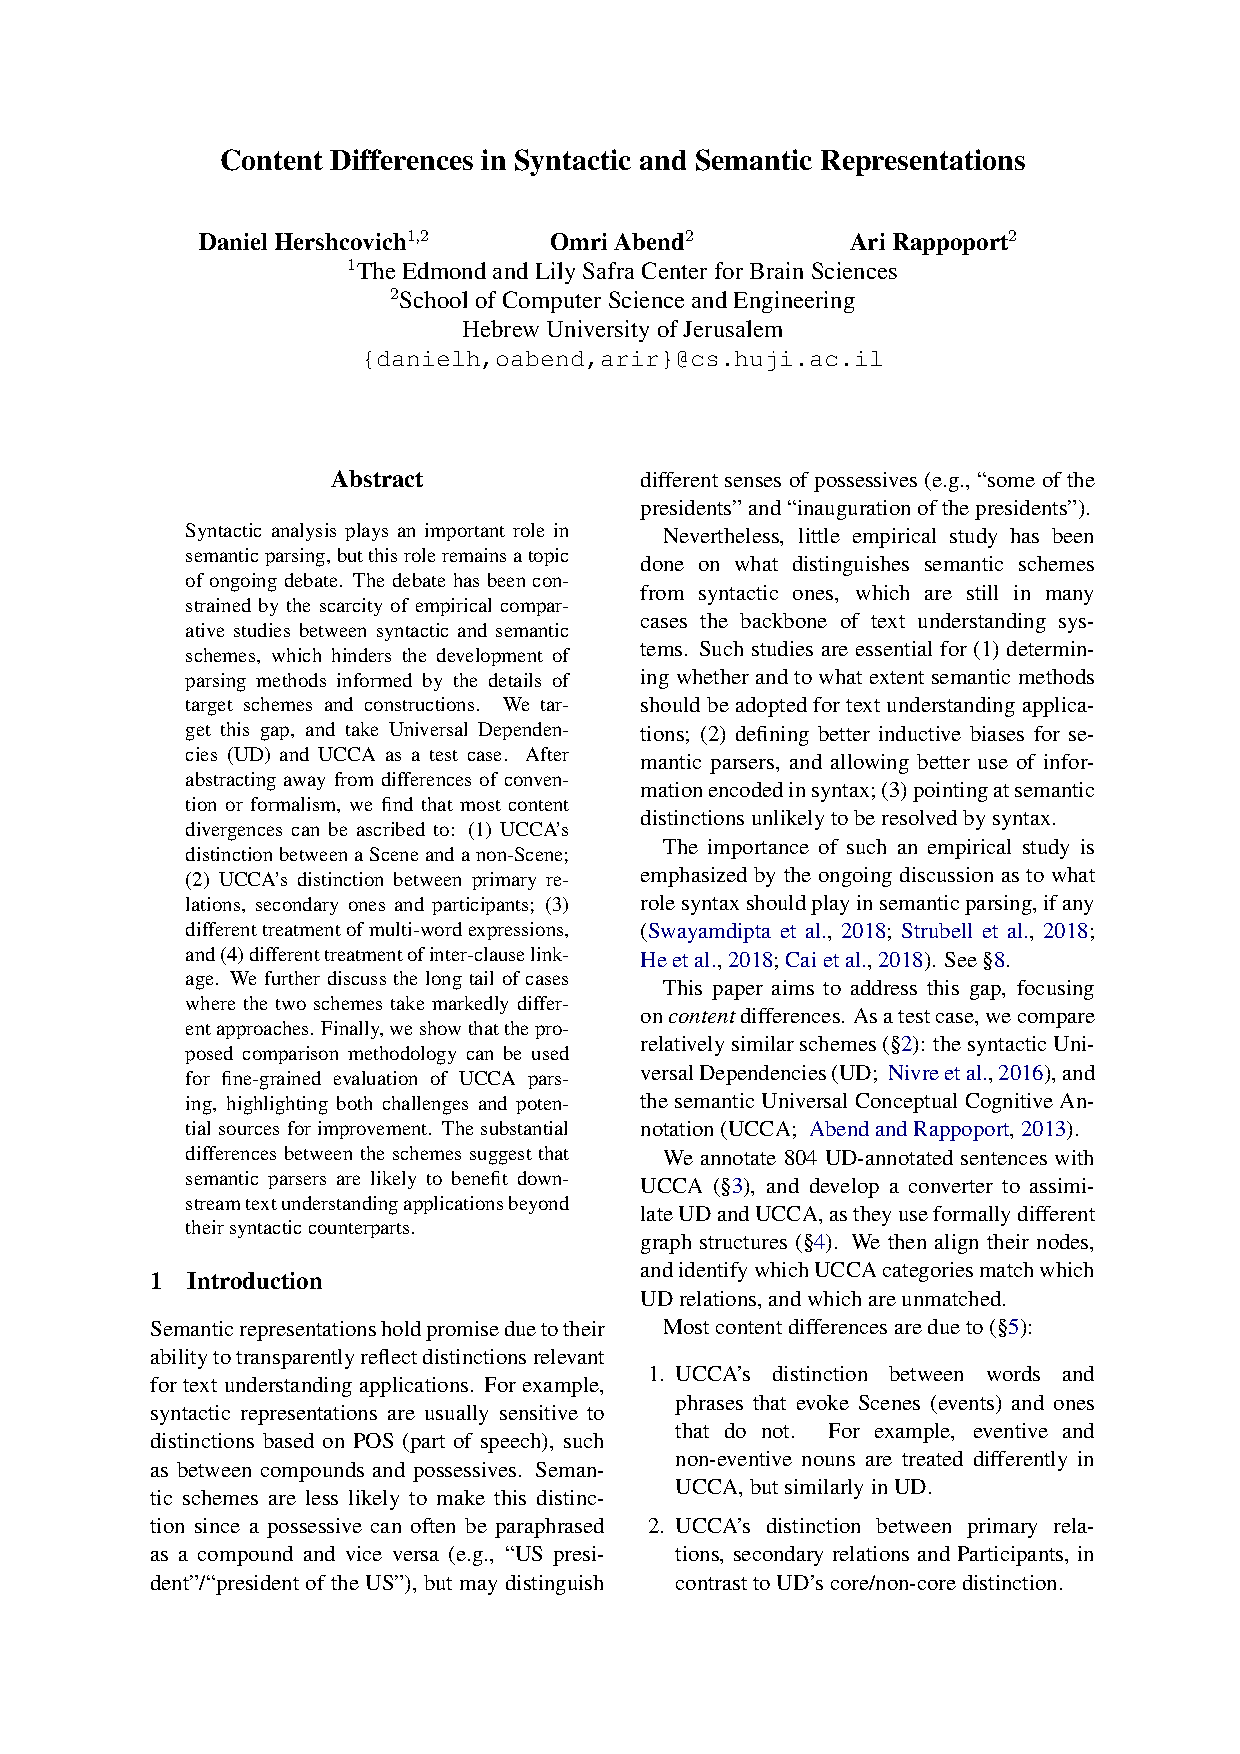
\includepdf[pages=-]{divergences.pdf}

\chapter*{Content Differences in Syntactic and Semantic Representation \\ Supplementary Notes}

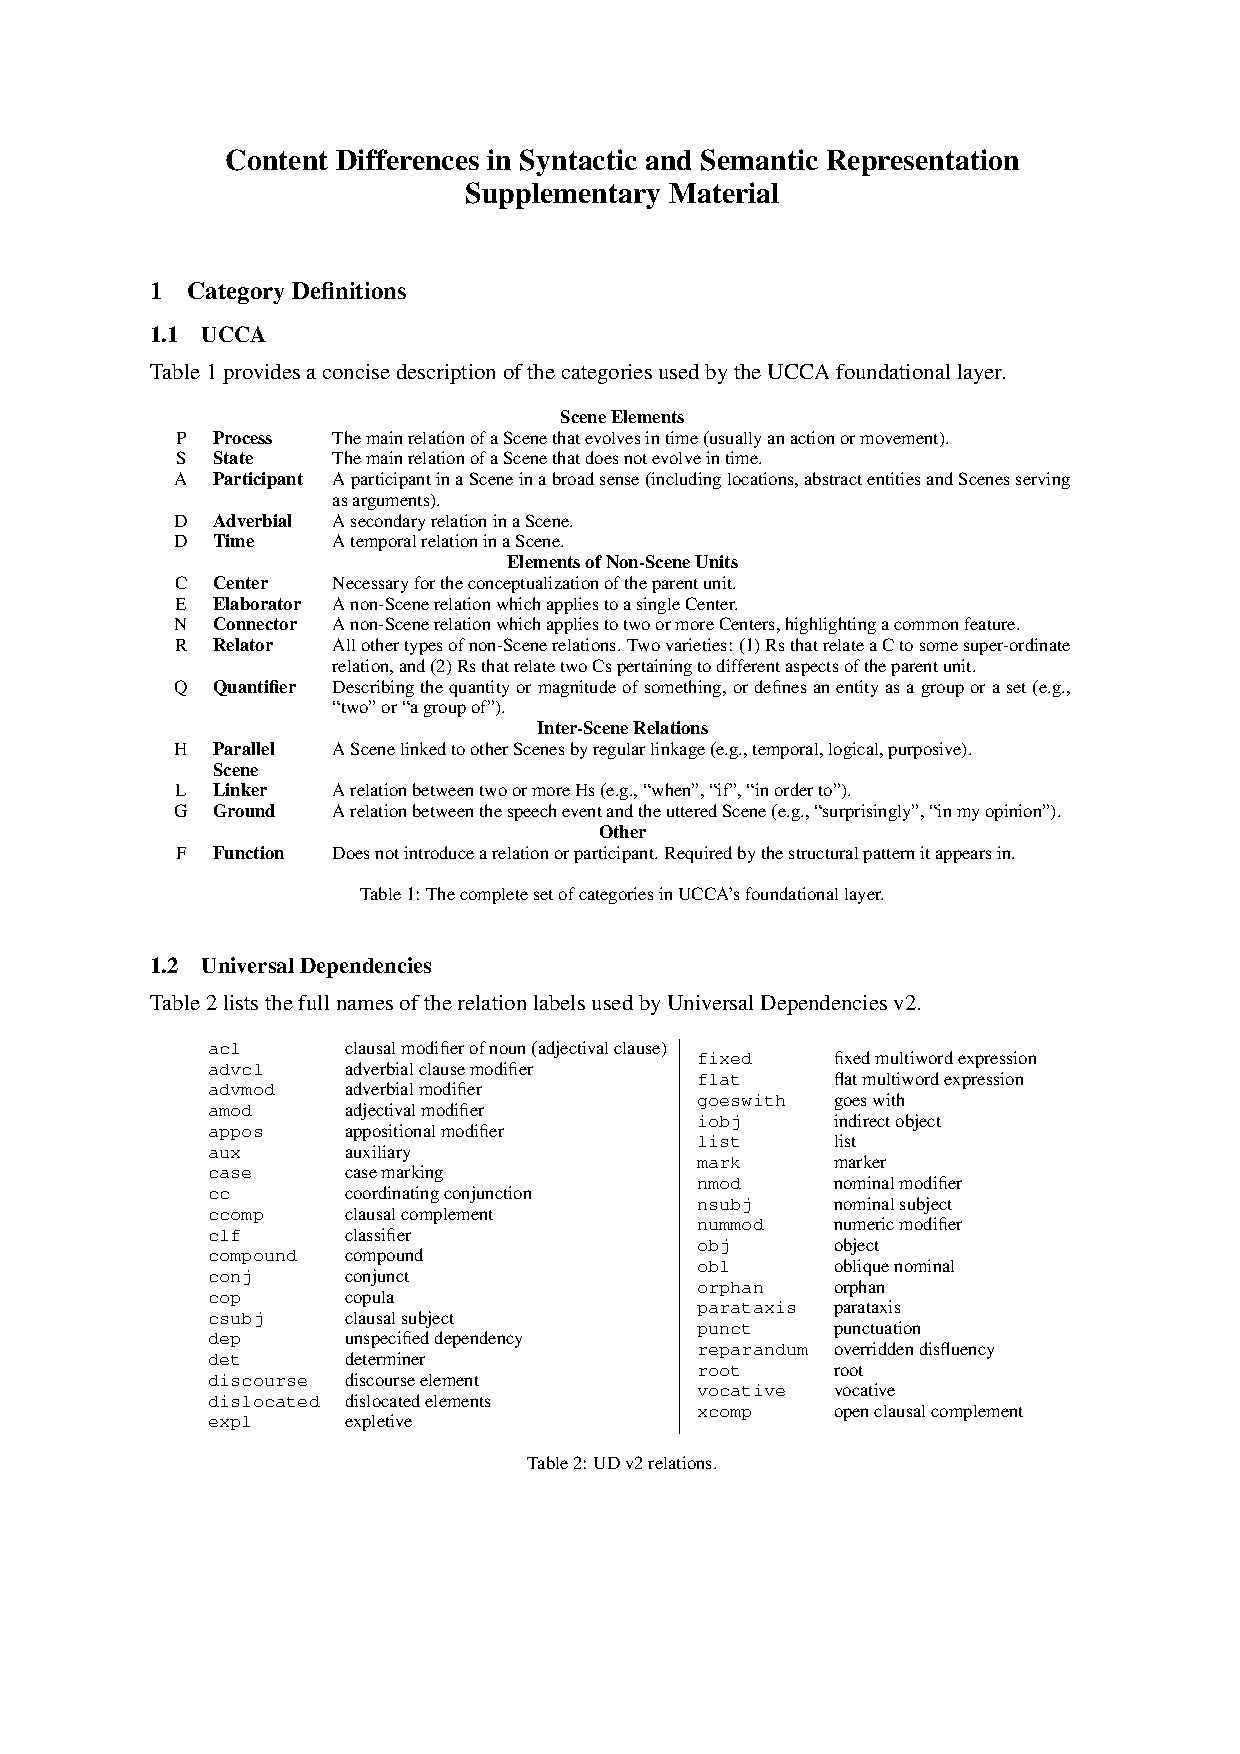
\includepdf[pages=-]{divergences_supp.pdf}




\chapter{Discussion}

In this thesis, I showed that meaning representation is valuable for language understanding,
and that TUPA, an accurate UCCA parser, is suited to many meaning representations.
Furthermore, multitask learning allows useful shared generalizations to emerge,
improving TUPA's performance by taking advantage of its general transition-based
architecture and flexible neural network classifier.
As different meaning representations capture many similar distinctions,
this approach proved effective, gaining from data annotated in each scheme
even though they had been designed separately and with different formal properties.
While divergences between the content of the schemes may limit the gain from sharing,
they highlight relative strengths, which are meaningful both theoretically and practically.

\section*{Challenges}

At the initial stages of this work, dataset size was a concern.
Models with a large number of parameters,
such as the neural network models employed in TUPA,
typically require very large training sets.
Since the UCCA datasets are small in relation to other schemes,
training neural network models on them seemed to pose a challenge.
However,
the current performance of TUPA in UCCA parsing is already quite satisfactory.
This is demonstrated by the fact that the parser has been successfully used in
various applications \cite{choshen2018reference,sulem2018semantic,sulem2018simple}.
Furthermore,
multitask learning proved to be an effective method to overcome the data scarcity issue.
The UCCA data has also been slowly growing and extended to more languages by further labeling efforts,
and results seem to improve as more and more training data is available.

While many distinctions are shared between UCCA and other semantic and syntactic schemes,
they are largely obscured by differences in representation format and convention.
A second challenge was thus in developing a generic parsing system that would be able
to handle more than one semantic scheme.
However, the general architecture of the parser was effective in handling these
graphs structure.
Conversion to a common graph format and assimilation of superficial structures
addressed the generality question effectively to allow multitask learning,
and further, allowed deep inspection of content divergences and convergences.

\section*{Impact}

UCCA's merits in providing a cross-linguistically applicable,
broad-coverage annotation will support ongoing efforts to incorporate deeper
semantic structures into a variety of applications, such as machine translation
\citep{jones2012semantics} and summarization \citep{liu2015toward}.
The advantage of UCCA as compared to syntactic annotation schemes for machine translation is apparent,
as translation tends to preserve semantic structure more than syntactic structure \citep{sulem2015conceptual}.
Using UCCA as an intermediate representation is thus likely to achieve outputs that are more
semantically similar to the source.

\subsection*{Benefit of Multitask Learning}

To further quantify the improvements due to multitask learning, where the tasks of parsing
multiple semantic representations are combined as auxiliary tasks for TUPA to improve UCCA
parsing, Figure~\ref{fig:fine_grained} offers a fine-grained analysis of the performance of different
multitask models.
The benefit of the multitask models over the single-task baseline is especially apparent for
Connectors and Linkers, demonstrating the improved capability to parse coordination structures
correctly, which are indeed relevant for all meaning representations.
Furthermore, while the labeled F1 for State is uniformly low due to the rarity of this category
and its common confusion with Process, the multitask model with all auxiliary task is able to reach
40\% labeled F1, showing it is able to generalize this difficult distinction between predicates
describing events and attributes.
In French and German, the improvement is again apparent for Connectors and Linkers,
but now especially also for Parallel Scenes---these seem to be responsible for most of the improvement
due to multitask learning in these languages.
Again, this shows that the syntactic ability to split phrases and clauses to separate Scenes is greatly
boosted by the auxiliary task (UD in this case).

Figure~\ref{fig:fine_grained_ud} shows fine-grained analysis by UD relations.
Surprisingly, determiners seem to suffer from multitask learning, as the single-task baseline does
best on them.
While determiners in UCCA are mostly Elaborators (in the version of the corpora on which the experiment
was made), they are mostly treated as vacuous semantically in DM and AMR, which could explain their
poor representation in models trained with these auxiliary tasks.
UD as an auxiliary greatly helps with this category in French and German, but also seems to deteriorate
its treatment in English.
Prepositions in German (bearing the case relation) are greatly improved by adding UD as an auxiliary.
This is a common relation, spread over multiple UCCA categories. Learning to represent it more accurately
improves performance across the board.


\pgfplotstableread{
category	single	UCCAAMR	UCCAUD	UCCADM	UCCADMUD	UCCAAMRUD	UCCAAMRDM	UCCAAMRDMUD
Participant	77	76	77	77	77	77	77	78
Center	78	77	77	78	80	78	79	79
Adverbial	78	75	77	77	75	76	75	75
Elaborator	77	77	77	78	78	79	79	78
ParallelScene	75	76	75	78	77	75	77	76
Connector	83	84	84	86	89	84	90	87
Relator	92	91	91	92	93	92	92	92
State	35	37	36	38	37	36	34	40
Function	82	82	80	83	84	85	83	84
Process	78	77	76	76	78	77	78	77
Linker	78	84	82	87	81	82	82	83
}\englishwiki
\pgfplotstableread{
category	single	UCCAUD
Participant	38	48
Center	77	76
Adverbial	25	32
Elaborator	21	26
ParallelScene	23	38
Connector	78	89
Relator	16	14
State	0	0
Function	67	68
Process	0	0
Linker	30	50
}\french
\pgfplotstableread{
category	single	UCCAUD
Participant	79	84
Center	89	90
Adverbial	66	72
Elaborator	87	89
ParallelScene	41	83
Connector	78	86
Relator	79	80
State	93	93
Function	0	0
Process	88	85
Linker	71	72
}\german


\pgfplotstableread{
category	single	UCCAAMR	UCCAUD	UCCADM	UCCADMUD	UCCAAMRUD	UCCAAMRDM	UCCAAMRDMUD
case	84	82	84	82	85	83	82	83
compound	83	84	87	81	83	81	81	78
iobj	85	82	83	84	82	83	84	86
nmod	85	84	85	86	88	85	84	87
nsubj	78	78	77	77	83	81	82	81
obj	88	84	84	88	93	87	86	91
appos	84	83	86	85	85	85	83	85
conj	76	80	78	81	80	81	80	81
det	82	67	59	53	67	67	47	57
acl	80	81	82	83	81	80	83	81
amod	81	83	86	86	86	84	86	83
}\englishwikiud
\pgfplotstableread{
category	single	UCCAAMR	UCCAUD	UCCADM	UCCADMUD	UCCAAMRUD	UCCAAMRDM	UCCAAMRDMUD
aux	84	83	83	85	86	84	84	86
obl	78	77	78	80	79	79	83	80
advcl	81	78	81	79	82	82	82	80
expl	64	65	60	63	62	62	59	69
mark	44	44	44	50	44	50	44	50
cc	80	93	80	93	93	93	93	93
advmod	83	83	82	86	84	85	85	83
nummod	84	90	94	87	81	90	84	94
ccomp	86	86	86	86	86	86	86	86
}\englishwikiudb
\pgfplotstableread{
category	single	UCCAUD
case	78	84
compound	22	32
iobj	10	18
nmod	34	51
nsubj	27	34
obj	19	38
appos	37	17
conj	26	31
det	87	89
acl	11	23
amod	48	51
aux	47	70
obl	27	41
advcl	13	14
expl	12	12
mark	29	36
cc	42	64
advmod	19	26
nummod	58	44
parataxis	0	27
cop	44	28
ccomp	10	41
xcomp	22	28
}\frenchud
\pgfplotstableread{
category	single	UCCAUD
case	6	82
compound	74	79
iobj	59	67
nmod	90	91
nsubj	95	96
obj	84	85
appos	89	92
conj	79	81
det	10	91
acl	65	72
amod	80	90
aux	62	63
obl	45	73
advcl	75	79
expl	74	76
mark	76	76
cc	73	76
advmod	53	62
nummod	76	74
parataxis	78	90
cop	90	91
ccomp	56	79
xcomp	67	67
}\germanud

\begin{figure}
\begin{subfigure}{\textwidth}
    \begin{tikzpicture}
    \begin{axis}[
    ybar=0pt,
    ymin=0,
    width=18cm,
    height=6cm,
    bar width=4pt,
    xtick=data,
    xticklabels from table={\englishwiki}{category},
    xticklabel style={font=\tiny,rotate=50,anchor=east},
    xtick align=inside,
    xticklabel pos=left,
    yticklabels=none,
    tickwidth=0pt,
    legend style={at={(axis cs:-1,100)},anchor=south west,font=\tiny,draw=none,legend columns=-1},
    legend cell align={left},
    nodes near coords={\scalebox{.4}{\pgfmathprintnumber[precision=2]{\pgfplotspointmeta}}},
    every node near coord/.append style={rotate=90,anchor=west}]
    \addplot[fill=green]table[x expr=\coordindex,meta=category,y=single]{\englishwiki};
    \addplot[fill=blue]table[x expr=\coordindex,meta=category,y=UCCAAMR]{\englishwiki};
    \addplot[fill=red]table[x expr=\coordindex,meta=category,y=UCCAUD]{\englishwiki};
    \addplot[fill=orange]table[x expr=\coordindex,meta=category,y=UCCADM]{\englishwiki};
    \addplot[fill=magenta]table[x expr=\coordindex,meta=category,y=UCCADMUD]{\englishwiki};
    \addplot[fill=cyan]table[x expr=\coordindex,meta=category,y=UCCAAMRUD]{\englishwiki};
    \addplot[fill=yellow]table[x expr=\coordindex,meta=category,y=UCCAAMRDM]{\englishwiki};
    \addplot[fill=brown]table[x expr=\coordindex,meta=category,y=UCCAAMRDMUD]{\englishwiki};
    \legend{Single,UCCA+AMR,UCCA+UD,UCCA+DM,UCCA+DM+UD,UCCA+AMR+UD,UCCA+AMR+DM,All}
    \end{axis}
    \end{tikzpicture}
    \caption{English Wiki}
\end{subfigure}
\begin{subfigure}{.475\textwidth}
    \begin{tikzpicture}
    \begin{axis}[
    ybar=0pt,
    ymin=0,
    width=9cm,
    height=6cm,
    bar width=4pt,
    xtick=data,
    xticklabels from table={\french}{category},
    xticklabel style={font=\tiny,rotate=50,anchor=east},
    xtick align=inside,
    xticklabel pos=left,
    yticklabels=none,
    tickwidth=0pt,
    nodes near coords={\scalebox{.4}{\pgfmathprintnumber[precision=2]{\pgfplotspointmeta}}},
    every node near coord/.append style={rotate=90,anchor=west}]
    \addplot[fill=green]table[x expr=\coordindex,meta=category,y=single]{\french};
    \addplot[fill=red]table[x expr=\coordindex,meta=category,y=UCCAUD]{\french};
    \end{axis}
    \end{tikzpicture}
    \caption{French 20K}
\end{subfigure}
\begin{subfigure}{.475\textwidth}
    \begin{tikzpicture}
    \begin{axis}[
    ybar=0pt,
    ymin=0,
    width=9cm,
    height=6cm,
    bar width=4pt,
    xtick=data,
    xticklabels from table={\german}{category},
    xticklabel style={font=\tiny,rotate=50,anchor=east},
    xtick align=inside,
    xticklabel pos=left,
    yticklabels=none,
    tickwidth=0pt,
    nodes near coords={\scalebox{.4}{\pgfmathprintnumber[precision=2]{\pgfplotspointmeta}}},
    every node near coord/.append style={rotate=90,anchor=west}]
    \addplot[fill=green]table[x expr=\coordindex,meta=category,y=single]{\german};
    \addplot[fill=red]table[x expr=\coordindex,meta=category,y=UCCAUD]{\german};
    \end{axis}
    \end{tikzpicture}
    \caption{German 20K}
\end{subfigure}
    \caption{TUPA's F1 per UCCA category in each single-/multitask setting.
    \label{fig:fine_grained}}
\end{figure}

\begin{figure}
\begin{subfigure}{\textwidth}
    \begin{tikzpicture}
    \begin{axis}[
    ybar=0pt,
    ymin=0,
    width=18cm,
    height=5cm,
    bar width=4pt,
    xtick=data,
    xticklabels from table={\englishwikiud}{category},
    xticklabel style={font=\tiny,rotate=50,anchor=east},
    xtick align=inside,
    xticklabel pos=left,
    yticklabels=none,
    tickwidth=0pt,
    legend style={at={(axis cs:-1,100)},anchor=south west,font=\tiny,draw=none,legend columns=-1},
    legend cell align={left},
    nodes near coords={\scalebox{.4}{\pgfmathprintnumber[precision=2]{\pgfplotspointmeta}}},
    every node near coord/.append style={rotate=90,anchor=west}]
    \addplot[fill=green]table[x expr=\coordindex,meta=category,y=single]{\englishwikiud};
    \addplot[fill=blue]table[x expr=\coordindex,meta=category,y=UCCAAMR]{\englishwikiud};
    \addplot[fill=red]table[x expr=\coordindex,meta=category,y=UCCAUD]{\englishwikiud};
    \addplot[fill=orange]table[x expr=\coordindex,meta=category,y=UCCADM]{\englishwikiud};
    \addplot[fill=magenta]table[x expr=\coordindex,meta=category,y=UCCADMUD]{\englishwikiud};
    \addplot[fill=cyan]table[x expr=\coordindex,meta=category,y=UCCAAMRUD]{\englishwikiud};
    \addplot[fill=yellow]table[x expr=\coordindex,meta=category,y=UCCAAMRDM]{\englishwikiud};
    \addplot[fill=brown]table[x expr=\coordindex,meta=category,y=UCCAAMRDMUD]{\englishwikiud};
    \legend{Single,UCCA+AMR,UCCA+UD,UCCA+DM,UCCA+DM+UD,UCCA+AMR+UD,UCCA+AMR+DM,All}
    \end{axis}
    \end{tikzpicture}
    \caption{English Wiki}
\end{subfigure}
\begin{subfigure}{\textwidth}
    \begin{tikzpicture}
    \begin{axis}[
    ybar=0pt,
    ymin=0,
    width=18cm,
    height=5cm,
    bar width=4pt,
    xtick=data,
    xticklabels from table={\englishwikiudb}{category},
    xticklabel style={font=\tiny,rotate=50,anchor=east},
    xtick align=inside,
    xticklabel pos=left,
    yticklabels=none,
    tickwidth=0pt,
    nodes near coords={\scalebox{.4}{\pgfmathprintnumber[precision=2]{\pgfplotspointmeta}}},
    every node near coord/.append style={rotate=90,anchor=west}]
    \addplot[fill=green]table[x expr=\coordindex,meta=category,y=single]{\englishwikiudb};
    \addplot[fill=blue]table[x expr=\coordindex,meta=category,y=UCCAAMR]{\englishwikiudb};
    \addplot[fill=red]table[x expr=\coordindex,meta=category,y=UCCAUD]{\englishwikiudb};
    \addplot[fill=orange]table[x expr=\coordindex,meta=category,y=UCCADM]{\englishwikiudb};
    \addplot[fill=magenta]table[x expr=\coordindex,meta=category,y=UCCADMUD]{\englishwikiudb};
    \addplot[fill=cyan]table[x expr=\coordindex,meta=category,y=UCCAAMRUD]{\englishwikiudb};
    \addplot[fill=yellow]table[x expr=\coordindex,meta=category,y=UCCAAMRDM]{\englishwikiudb};
    \addplot[fill=brown]table[x expr=\coordindex,meta=category,y=UCCAAMRDMUD]{\englishwikiudb};
    \end{axis}
    \end{tikzpicture}
    \caption{English Wiki (cont.)}
\end{subfigure}
\begin{subfigure}{\textwidth}
    \begin{tikzpicture}
    \begin{axis}[
    ybar=0pt,
    ymin=0,
    width=18cm,
    height=5cm,
    bar width=4pt,
    xtick=data,
    xticklabels from table={\frenchud}{category},
    xticklabel style={font=\tiny,rotate=50,anchor=east},
    xtick align=inside,
    xticklabel pos=left,
    yticklabels=none,
    tickwidth=0pt,
    nodes near coords={\scalebox{.4}{\pgfmathprintnumber[precision=2]{\pgfplotspointmeta}}},
    every node near coord/.append style={rotate=90,anchor=west}]
    \addplot[fill=green]table[x expr=\coordindex,meta=category,y=single]{\frenchud};
    \addplot[fill=red]table[x expr=\coordindex,meta=category,y=UCCAUD]{\frenchud};
    \end{axis}
    \end{tikzpicture}
    \caption{French 20K}
\end{subfigure}
\begin{subfigure}{\textwidth}
    \begin{tikzpicture}
    \begin{axis}[
    ybar=0pt,
    ymin=0,
    width=18cm,
    height=5cm,
    bar width=4pt,
    xtick=data,
    xticklabels from table={\germanud}{category},
    xticklabel style={font=\tiny,rotate=50,anchor=east},
    xtick align=inside,
    xticklabel pos=left,
    yticklabels=none,
    tickwidth=0pt,
    nodes near coords={\scalebox{.4}{\pgfmathprintnumber[precision=2]{\pgfplotspointmeta}}},
    every node near coord/.append style={rotate=90,anchor=west}]
    \addplot[fill=green]table[x expr=\coordindex,meta=category,y=single]{\germanud};
    \addplot[fill=red]table[x expr=\coordindex,meta=category,y=UCCAUD]{\germanud};
    \end{axis}
    \end{tikzpicture}
    \caption{German 20K}
\end{subfigure}
    \caption{TUPA's F1 per UD relation in each single-/multitask setting.
    \label{fig:fine_grained_ud}}
\end{figure}


\section*{Ongoing Work}

The ideas presented in this thesis offer many exciting opportunities for further research.
Following are two such directions, which I have started pursuing.

\subsection*{Combining Syntax with Lexical Semantics}

In the comparison between Universal Dependencies (UD) and UCCA,
88\% of edges were found to be common between the schemes (ignoring the label),
meaning the linguistic structures annotated by them are very similar.
Inspecting the remaining divergences reveals, for example, that only
about 82\% of UCCA unanalyzable units (i.e., units without a compositional
internal structure) are even sub-trees in UD.
The remaining cases seem to be almost exclusively multi-word Linkers,
such as ``even though'', ``when it comes to'' and ``just because''.
Furthermore, only 73\% of Participants in UCCA Scenes were found to be arguments
of syntactic predicates in UD, due to the differences in distinctions between
Scenes/non-Scenes and between main relations, secondary relations and participants.

These gaps can perhaps be closed
by complementing syntax with \textit{lexical} semantics to make up for differences
corresponding to semantic distinctions that are not expressed in UD.
Lexical semantic resources, such as STREUSLE
\citep{schneider-thesis,envmwe,pssdisambig,gensuper},
may provide the necessary annotation to close the gap between UD and UCCA:
for example, it contains labels for various types of multi-word expressions,
even ones that are not UD sub-trees;
and semantically categorize lexical items according to lexical category and
supersense, distinguishing, for example, eventive from non-eventive nouns.

\subsection*{Establishing the Meaning Representation Parsing Task}

TUPA, the parser presented in this thesis, is the first UCCA parser.
In other parsing tasks, years of experiments and progress have yielded very
accurate and fine-tuned parsers.
While TUPA is quite accurate, there can doubtlessly be countless improvements
due to different ways of looking at the problem or a better selection of architecture
and parameters.
During January 2019, we (Zohar Aizenbud, Leshem Choshen, Elior Sulem, Omri Abend,
Ari Rappoport and myself) ran a shared task as part of the
International Workshop on Semantic Evaluation, titled
Task 1: Cross-lingual Semantic Parsing with UCCA.
The task presented participants with UCCA parsing challenges
in English, German and French.
The shared task has yielded improvements over TUPA
in all languages and settings,
with various approaches with respect to the parsing system,
machine learning architecture, and cross-lingual
transfer.\footnote{\url{https://competitions.codalab.org/competitions/19160}}
The task results will be presented during SemEval
2019.\footnote{\url{http://alt.qcri.org/semeval2019/}}

More recently, a proposal for another shared task at
The SIGNLL Conference on Computational Natural Language
Learning\footnote{\url{http://www.conll.org/}} was accepted for CoNLL 2019.
The task, organized jointly by Stephan Oepen, Omri Abend, Jan Haji\v{c},
Tim O'Gorman, Nianwen Xue and myself,
will involve parsing into a range of different semantic representation schemes
(DM, PSD, EDS, UCCA and AMR), differing in both formal structure and linguistic
approaches.
By combining the different schemes in a single task, we
establish cross-framework meaning representation parsing as a task,
and hope to ``blur the boundaries'' and enable cross-fertilization between
meaning representations.

To conclude, I see learning semantic parsing as a means for computers to learn language.
While different representations focus on different distinctions and do so
with formally different structures, they share an overall goal,
which is to support both natural language processing applications and linguistic
theory.
The combined datasets annotated in each of these representations are an invaluable
resource, which, used effectively, can greatly boost our achievements in
language understanding and processing.

\bibliography{references}
\bibliographystyle{apalike}

\pagebreak

\section*{\flushright{\heb{תקציר}}}

\begin{flushright}
\heb{עיבוד שפה טבעית הוא תחום מדעי וטכנולוגי העוסק בפיתוח שיטות לביצוע משימות לשוניות בצורה אוטומטית.
אלו כוללות סיווג טקסט לקטגוריות, תיוג לפי תכונות בלשניות )כמו למשל חלקי דיבר(,
בניית ייצוגים גרפיים עבורו וייצור טקסט חדש לפי אילוצים מסויימים.
למשל, בתרגום מכונה יש לייצר טקסט חדש בשפת יעד בהנתן טקסט בשפת המקור.}

\heb{מאמץ רב בעיבוד שפה טבעית מוקדש להבנת שפה טבעית, תחום אשר שם לעצמו כמטרה להיות מסוגל להבין טקסט,
להקיש ממנו היסקים, ולפעול על פיו באופן מלומד. בעוד לשימושים מסויימים ניתן להשתמש בשיטות פשוטות יחסית,
אשר מתעלמות לחלוטין מסדר המלים )מודלים מסוג שק מלים( או מתייחסות אליו כשרשרת פשוטה
)כמו שיטת הרצף-לרצף הנפוצה, המאפשרת לרשתות נוירונים ללמוד משימות באופן כולל(, הבנת טקסט באופן כללי דורשת
ייצוג היררכי של משמעות. בניית ייצוג זה מהטקסט היא מטרתה של סדרת עבודות רחבה בתחום הניתוח הסמנטי.
בעוד ייצוגים סמנטיים רבים הוצעו עד כה, יש ביניהם הרבה מן המשותף בנוגע לאבחנות הבסיסיות, כמו למשל בין
פרדיקטים )יחסים, מצבים ואירועים( ובין ארגומנטים )משתתפים(.}

\heb{תזה זו מתמקדת בייצוג סמנטי מסויים בשם ACCU, אשר העקרונות המנחים העיקריים שלו הם
תמיכה בכל התופעות הלשוניות הסמנטיות, תמיכה ויציבות בין שפות, קלות התיוג )אפילו בידי מי שאינו מומחה בבלשנות(,
וארכיטקטורה מודולרית התומכת בשכבות שונות של אנוטציה סמנטית.
מנתח אוטומטי לחלוטין מוצע במסגרת התזה, ומוערך על פני מספר שפות )אנגלית, צרפתית וגרמנית(.
המנתח, אשר שמו APUT, מסוגל ללמוד מבנים גרפיים כללים ביותר: גרפים מכוונים חסרי מעגלים על-פני
סדרות של מלים עם צמתים פנימים עבור יחידות מורכבות, אשר יכולים לכסות סדרות לא רצופות של מלים.
המחלקה הכללית הזו של גרפים מכסה את המבנים אשר מתוייגים ב-ACCU, וגם ייצוגים אחרים.
APUT ממומש כמנתח מבוסס מעברים, אשר מערכת המעברים שלו תומכת בתכונות המבניות הללו.
מסווג המעברים של APUT הוא רשת נוירונים בעלת רכיב MTSLiB לחישוב ייצוגים עבור הקלט.
בהשוואה נרחבת לעומת שיטות המבוססות על המרה למבנים פשוטים יותר, וגם בהשוואה למימושים אחרים של המסווג,
נמצא ש-APUT מסוגל לנתח בדיוק רב יותר טקסט למבני ACCU, גם במצב שבו אוסף הבדיקה דומה לאוסף האימון
וגם כאשר הוא נלקח ממקור שונה. תוצאות אלו תקפות לשלוש שפות.}

\heb{יכולתו של המנתח מודגמת גם לשתי שיטות אחרות לניתוח סמנטי, MD ו-RMA,
וגם לניתוח תחבירי בשיטת DU. ניסוי זה מדגים את גמישותו של המנתח, ואת יכולתו להתמודד
עם משימות נוספות מלבד ACCU. בנוסף, כאשר מאמנים את APUT על מספר משימות בעת ובעונה אחת,
ביצועיו משתפרים על ACCU. שיפור זה נעשה באמצעות למידה של הכללות הנוגעות לכל המשימות וחשובות להן.}

\heb{לבסוף, בהשוואה אמפירית של התוכן בייצוגים סמנטיים ותחביריים, אנו מגלים פנים שונים של הבדל ביניהם.
להבדלים אלו יש משמעות רבה בנוגע לתרומה של תחביר לניתוח סמנטי, ועל השימושיות של כל אחת מהשיטות למשימות
סמנטיות בעיבוד שפה טבעית.}
\end{flushright}

\pagebreak

\clearpage

\title{}
\author{
\heb{עבודה זו נעשתה בהדרכתם של} \\
\heb{פרופ' ארי רפופורט וד"ר עמרי אבנד}}
\date{}

\maketitle
\clearpage

\title{
\textbf{\heb{ניתוח סמנטי אוניברסלי באמצעות רשתות נוירונים}} \\
\vspace{2cm}
{\large\heb{חיבור לשם קבלת תואר דוקטור לפילוסופיה}}
}
\author{
\heb{מאת}\\
\heb{דניאל הרשקוביץ}
\vspace{2cm}
}
\date{
\heb{הוגש לסנט האוניברסיטה העברית בירושלים} \\
\heb{פברואר 9102}
}

\maketitle
\maketitle

\end{document}
